\begin{par}

    \begin{figure}[H]
        \centering
        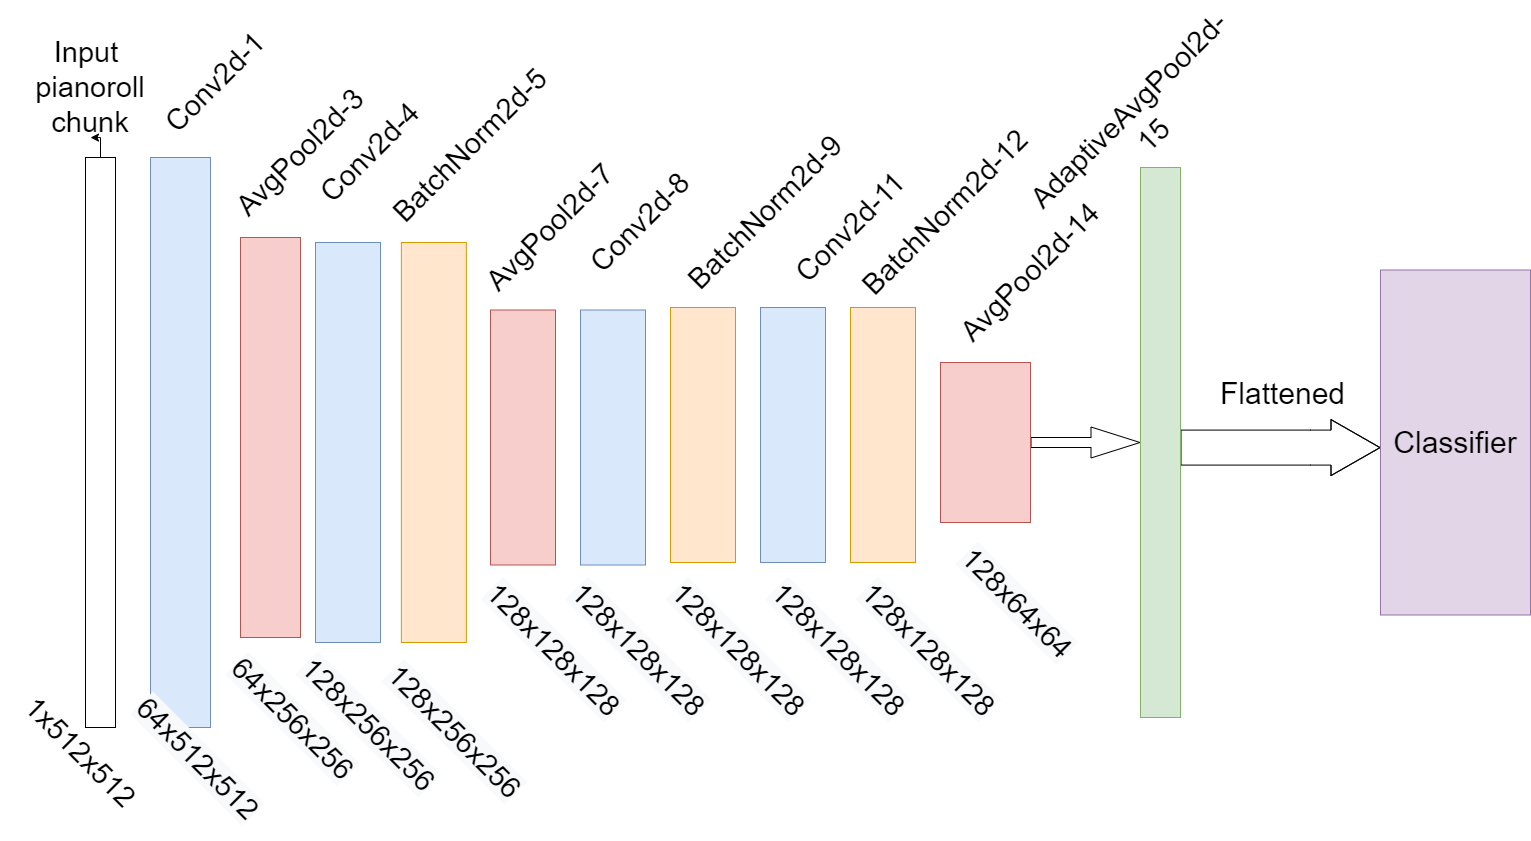
\includegraphics[width=4in]{image/cnn_classifier_feature_architecture}
        \caption{The feature extraction architecture of the CNN classifier}
        \label{fig:cnn_feature}
    \end{figure}

    \par \hspace{15pt} The first classification method the group proposed is a convolutional neural network (CNN) based classifier. The CNN classifier is based on the VGG-16 architecture, featuring convolution layers with small $3 \times 3$ filters. However to adapt the binary nature of the pianoroll, the team decided to replace the max pooling layers into average pooling layers to introduce more structural properties of the data as induction for the model. A more specific architecture will be discussed in the next several paragraphs.

    \par \hspace{15pt} Figure \ref{fig:cnn_feature} shows the feature extraction architecture of the CNN classifier. The feature extraction is done by convolutional layers stride of 2 and padding of $1$. We decided not to pad the input too much to maintain the structure of the binary data. The average pooling layers all have a kernel size of $2$ and stride of $2$ with no padding. The non-linear layer used in the feature extractor was ReLU. 
    
    \begin{figure}[H]
        \centering
        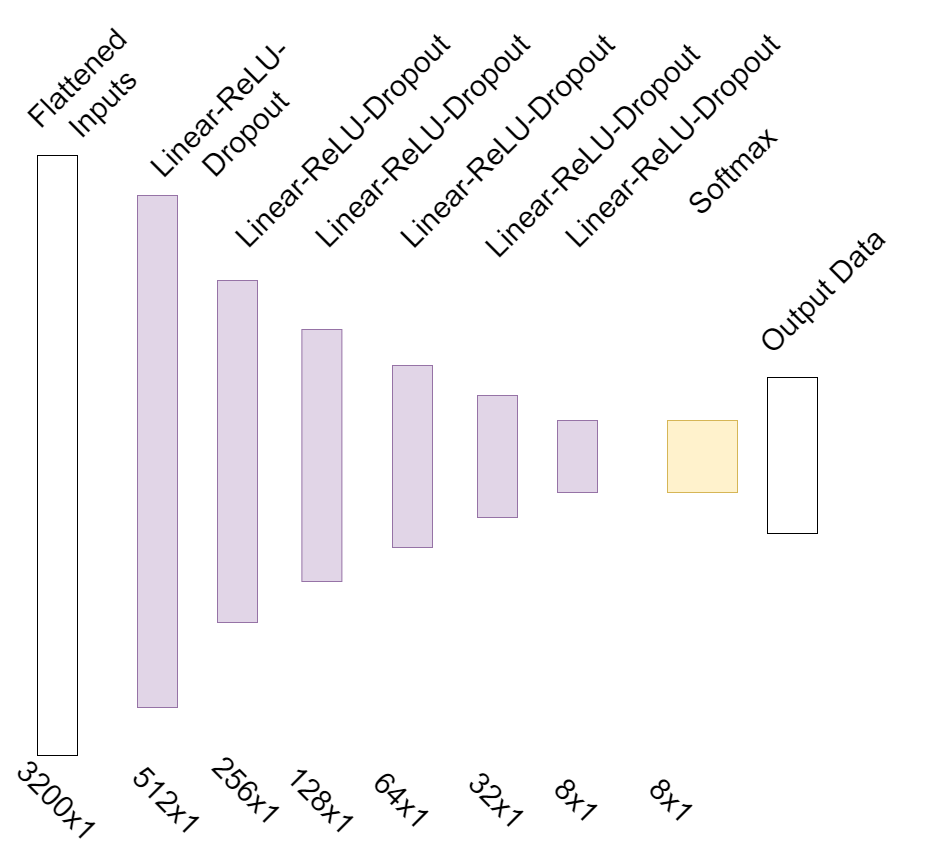
\includegraphics[width=4in]{image/cnn_classifier_architecture}
        \caption{Linear Classifier of the CNN classifier}
        \label{fig:cnn_class}
    \end{figure}
    
    \par \hspace{15pt} The output of the convolutional layers are pooled into a single vector. The output of the pooling layer is fed into a linear classifier, which is shown in Figure \ref{fig:cnn_class}. Dropout layers in the linear classifier shares a probability of $0.3$. Since we believe that can be used to prevent overfitting due to the small training set. In the end, the output of the linear-ReLU-Dropout layers was fed into a softmax layer for classification.

\end{par}